%------------------------ Torsion Springs -------------------------%
\subsection{Torsion Springs} \label{subsec:Tspring}

%------------------------------ Inputs and Outputs ------------------------------%
\subsubsection{Inputs and Outputs}
Each leg's motor shafts have a pair of torsion springs to compensate for the backdrivability of the harmonic drives. The idea is to limit the torque to a value beneath the harmonic drive's backdrivable torque when it is not powered. The inputs are then the maximum torque generated at the knee $M_{knee\ max} = 32.36\text{ MPa}$ and the maximum torque generated at the hip $M_{hip\ max} = 47.44\text{ MPa}$ from Figure \ref{fig:mod_torque_cycle} in Section \ref{sec:stability}. Additionally, the minimum torques $M_{knee\ min} = 19.08\text{ Nm}$ and $M_{hip\ min} = 31.07\text{ Nm}$ are used to ensure that the minimal deflection angles of the torsion springs provide sufficient torques based on the angular positions of the limbs. The tibia span ($\theta_{tibia\ max}-\theta_{tibia\ min}$) approaches $45^{\circ}$ while the thigh span ($\theta_{thigh\ max}-\theta_{thigh\ min}$) is only about $25^{\circ}$. Also, the outer diameters of the spacers ($D_{knee\ spacer} = 31.5\text{ mm}$, $D_{hips\ spacer} = 33.5\text{ mm}$) are given to ensure that all torsion springs do not interfere with the shaft spacers when deflected.

The torsion spring analysis will generate many outputs such as the various dimensions of the springs. However, the most important outputs are the spring constants $k_{knee}$ and $k_{hip}$ that are used to compute the resultant torques taken by both harmonic drives.
%------------------------------ CONSTANTS ------------------------------%
\subsubsection{Constants and Parameters}
The spring free angle $\beta$ can vary between $90^{\circ}$ and $360^{\circ}$, but a value of $\beta = 90^{\circ}$ was set to be a constant for the purpose of this analysis. Similarly, the number of full turns made by the spring coil was chosen to be $N_f = 3$ turns. The length arms were kept constant for both springs ($l_{1\ knee} = l_{2\ knee} = 25\text{ mm}$, $l_{1\ hip} = l_{2\ hip} = 25\text{ mm}$).
%------------------------------ Assumptions ------------------------------%
\subsubsection{Assumptions and Simplifications}
It is assumed that the backdriving torque of a harmonic drive corresponds to approximately 1/5 of the harmonic drive's rated torque based on the data sheets presented in Appendix \ref{app:datasheets}. For this purpose, it is also assumed that the rated torque of the harmonic drive coincides with the maximum torques $M_{knee\ max}$ and $M_{hip\ max}$. 
\begin{equation}
    M_{knee\ bd} \simeq \frac{M_{knee\ max}}{5} = \frac{32.36\text{ MPa}}{5}= 6.47\text{ MPa}
\end{equation}
\begin{equation}
    M_{hip\ bd} \simeq \frac{M_{hip\ max}}{5} = \frac{47.44\text{ MPa}}{5} = 9.45\text{ MPa}
\end{equation}
Two torsion springs equally share the torque in such a way that the maximum and minimum torque generated by a single torsion spring can be obtained as follows.
\begin{equation}
    M_{max\ hip\ spring} \geq \frac{1}{2}(M_{hip\ max} - M_{hip\ bd}) = \frac{1}{2} \frac{4}{5}M_{hip\ max} = \frac{4}{10}(47.44\text{ Nm}) = 18.98\text{ Nm}
\end{equation}
\begin{equation}
    M_{min\ hip\ spring} \geq \frac{1}{2}(M_{hip\ min} - M_{hip\ bd}) = \frac{1}{2} (31.07\text{ Nm} - 9.45\text{ MPa}) = 10.79\text{ Nm}
\end{equation}
%------------------------------ Materials ------------------------------%
\subsubsection{Material Selection}
The chosen material for all springs is music wire due to it being a common spring material and also due to it's sufficient tensile strength for this application. The Young's Modulus $E$ of music wire, and most carbon steels, was given as $207\text{ GPa}$. The tensile strength $S_{ut}$ was obtained with the following constants $A$ and $m$, and a wire diameter $d$ of 6 mm in the equation below \cite{budynas_shigleys_2015}.
\begin{equation}
    S_{ut} = \frac{A}{d^m} = \frac{2211\text{ MPa\ mm}^{0.145}}{(6\text{ mm})^{0.145}} = 1705\text{ MPa}
\end{equation}
Then, for a music wire, the normal yield strength $S_y$ can be obtained with the following equation \cite{budynas_shigleys_2015}.
\begin{equation}
    S_y = 0.78S_{ut} = 0.78(1705\text{ MPa}) = 1330\text{ MPa}
\end{equation}
%------------------------------ Free-Body Diagram ------------------------------%
\subsubsection{Free-Body Diagram}
The analysis presented below covers the procedure followed to obtain the spring constant of the two torsion springs mounted on the hip shaft assembly. One of the two torsion spring is right-handed and the free-body diagram is presented on Figure \ref{fig:HipSpring}. The other spring is left-handed and is simply a mirrored version of the right-handed one.
\begin{figure}
    \centering
    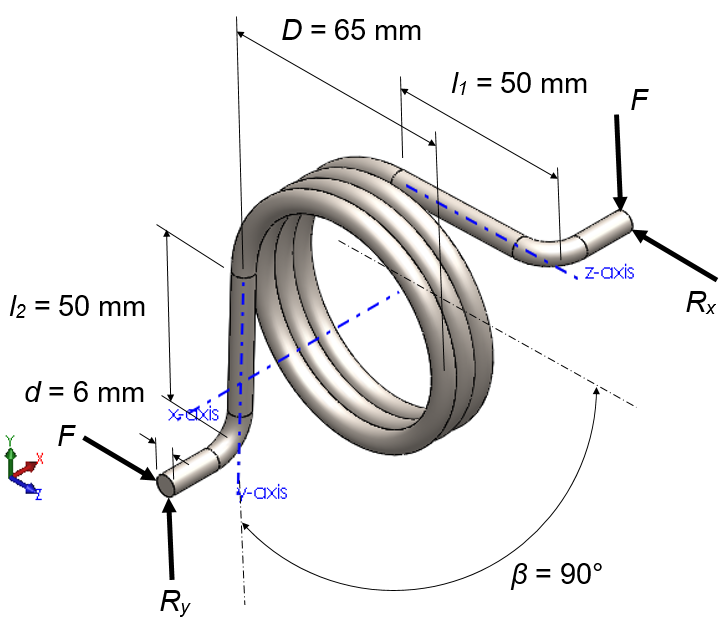
\includegraphics[width=0.5\textwidth]{4_Analysis/img/Spring/Hip_Spring_Ann.PNG}
    \caption{Hip right-handed torsion spring FBD}
    \label{fig:HipSpring}
\end{figure}
%------------------------------ Stress Analysis ------------------------------%
\subsubsection{Stress Analysis}
First, the maximum and minimum torque generated by the spring can be expressed as follows.
\begin{align}
    M_{max\ hip\ spring} \leq k_{min}\theta_{thigh\ max} && M_{min\ hip\ spring} \leq k_{min}\theta_{thigh\ min}
\end{align}
Where $k_{min}$ is the minimal spring constant necessary to reduce the harmonic drive torque below its backdrivable torque. Then, subtracting the second equation from the first isolating $k_{min}$ produces:
\begin{equation}
    k_{min} \geq  \frac{M_{max\ hip\ spring} - M_{min\ hip\ spring}}{k\theta_{thigh\ max} - k\theta_{thigh\ min}} = \frac{18.98\text{ Nm} - 10.79\text{ Nm}}{25^{\circ}\frac{\pi}{180^{\circ}}} = 18.76\text{ Nm}
\end{equation}
This signifies that the spring should be designed in such a way that $k_{min} \geq 18.76\text{ Nm}$. Now, to obtain the minimum and maximum spring deflections:
\begin{equation}
    \theta_{thigh\ max} \geq \frac{M_{max\ hip\ spring}}{k_{min}} = \frac{18.98\text{ Nm}}{18.76\text{ Nm}} = 1.01\text{ rad}\ \frac{180^{\circ}}{\pi} = 57.96^{\circ}
\end{equation}
\begin{equation}
    \theta_{thigh\ min} \geq \frac{M_{min\ hip\ spring}}{k_{min}} = \frac{10.79\text{ Nm}}{18.76\text{ Nm}} = 0.58\text{ rad}\ \frac{180^{\circ}}{\pi} = 32.96^{\circ}
\end{equation}
The next steps consisted of finding the spring specifications that would not only provide a valid spring constant but also limit the bending stress to the calculated yield stress. This process was done by trial and error for this report, but it will be part of the parameterization as explained in the Parameterization section.

First, based on the free angle $\beta$ of the spring, a linear function was quickly obtained to compute the number of partial turns $N_p$.
\begin{equation}
    N_p = -\frac{1}{360^{\circ}}\beta + 1 = -\frac{90^{\circ}}{360^{\circ}} + 1 = 0.25\text{ turn}
\end{equation}
Then, the number of body turns $N_b$ and number of active turns $N_a$ can be obtained. Equations \ref{eq:spring_first} to \ref{eq:spring_last} came from Shigley's textbook \cite{budynas_shigleys_2015}. 
\begin{equation}\label{eq:spring_first}
    N_b = N_f + N_p = 3\text{ turns} + 0.25\text{ turn} = 3.25\text{ turns}
\end{equation}
\begin{equation}
    N_a = N_b +\frac{l_1 + l_2}{3\pi D} = 3.25\text{ turns} +\frac{50\text{ mm} + 50\text{ mm}}{3\pi (65\text{ mm})} = 3.41\text{ turns}
\end{equation}
The shaft analysis from Section \ref{subsec:shaft} required the length occupied by the spring over the shaft. This length can be approximated as follows by using the wire diameter $d$ as a pitch value, and by not taking into consideration the length of the arms.
\begin{equation}
    L_{spring} \simeq N_a d = (3.41\text{ turns})(6\text{ mm/turn}) = 20.48\text{ mm}
\end{equation}
Then, to obtain the spring constant $k$ in torque per radian: 
\begin{equation}
    k =\frac{M}{\theta_t} = \frac{d^4 E}{64 D N_a} = \frac{(6\text{ mm})^4\ 207\times 10^3\text{ MPa}}{64 (65\text{ mm})(3.41 \text{ turns})}= 18.89\times 10^3\text{ Nmm/rad}
\end{equation}
The minimal value for $k_{min}$ can be compared with computed value for $k$ based of the dimensions of the spring.
\begin{equation}
    k = 18.89\text{ Nm/rad} > 18.76\text{ Nm/rad} = k_{min} 
\end{equation}
%\begin{equation}
%    k' = \frac{d^4 E}{10.8 D N_a} = \frac{(6\text{ mm})^4\ 207\times 10^3\text{ MPa}}{10.8 (50\text{ mm})(3.46 \text{ turns})}= 143.49\times 10^3\text{ Nmm/turn}
%\end{equation}
Now, to verify that the spring's inner coil diameter does not interfere with the spacer, the maximum bending moment was obtained with a maximum deflection $\theta_{max} = 58^{\circ}$.
\begin{equation}
    M_{max} = k(\theta_{max}-\theta = (18.89\times 10^3\text{ Nmm/rad})(58^{\circ}\frac{\pi}{180^{\circ}})= 19.13\times 10^3\text{ Nmm}
\end{equation}
Then, the angular deflection of the coil body in number of turns $\theta_c'$ and the final coil diameter $D'$ as well as the final inner diameter of the coil $D_i'$ can be obtained as follows.
\begin{equation}
    \theta_c' = \frac{10.8 M D N_b}{d^4 E} = \frac{10.8 (19.13\times 10^3\text{ Nmm})(65\text{ mm})(3.25\text{ turns})}{(6\text{ mm})^4\ 207\times 10^3\text{ MPa}}= 0.163\text{ turn}
\end{equation}
\begin{equation}
    D' = \frac{N_b D}{N_b + \theta_c'} = \frac{(3.25\text{ turns})(65\text{ mm})}{3.25\text{ turns}+0.163\text{ turn}}= 61.90\text{ mm}
\end{equation}
\begin{equation}
    D_i' = D' - d = 61.90\text{ mm} - 6\text{ mm} = 55.90\text{ mm}
\end{equation}
For this case, the minimum inner coil diameter is well above the spacer diameter $D_{hips\ spacer} = 33.5\text{ mm}$ and therefore, both components should not interfere. The last set of steps consist of obtaining the safety factor for the spring with the previous dimensions used. First, the stress-correction factor $K_i$ was obtained before computing the bending stress $\sigma$. Here, $C$ is the spring index which correlates to the ratio $D/d$ for torsion springs. Here, $C= 65\text{ mm}/6\text{ mm} = 10.83$ which is acceptable since it is recommended that $4 \leq C \leq 12$ \cite{budynas_shigleys_2015}.
\begin{equation}
    K_i = \frac{4C^2-C-1}{4C(C-1)} =  \frac{4(10.83)^2-10.83-1}{4(10.83)(10.83-1)} = 1.07
\end{equation}
\begin{equation}
    \sigma = K_i \frac{32 M}{\pi d^3} = 1.07 \frac{32 (19.13\times 10^3\text{ Nmm})}{\pi (6\text{ mm})^3} = 968.59 \text{ MPa}
\end{equation}
\begin{equation}\label{eq:spring_last}
    SF = \frac{S_y}{\sigma} = \frac{1330\text{ MPa}}{968.59\text{ MPa}} = 1.37 
\end{equation}
%------------------------------ Critical Review ------------------------------%
\subsubsection{Critical Review}
The dimensions of the springs obtained above are reasonable considering that the spring index $C$ of 10.83 is between the recommended range $4 \leq C \leq 12$ \cite{budynas_shigleys_2015}. Also, for a music wire, the wire diameter can go up to $6.5 \text{ mm}$ according to Shigley's textbook \cite{budynas_shigleys_2015}. However, trying to find a spring with such dimensions on various manufacturers' catalogues did not yield satisfying results.

The other set of torsion springs for the knee drive that were not presented in the stress analysis above were also computed. Here are the main results: free angle $\beta = 90^{\circ}$, wire diameter $d = 5\text{ mm}$, coil diameter $D = 40\text{ mm}$, arm length $l = 25\text{ mm}$, number of body turns $N_b = 3.25\text{ turns}$. The spring constant $k$ was found to be $14940\text{ Nmm/rad}$, the maximum deflection $\theta_{max}$ chosen as $88^{\circ}$ which yields a maximum torque $M_{max}$ of $26672.75\text{ Nmm}$ while respecting a safety factor of 1.16. Now, two graphs comparing the resulting torques that the harmonic drives have to hold before and after the addition of the spring are presented on Figure \ref{fig:TorqueB4&after}

\begin{figure}
    \centering
    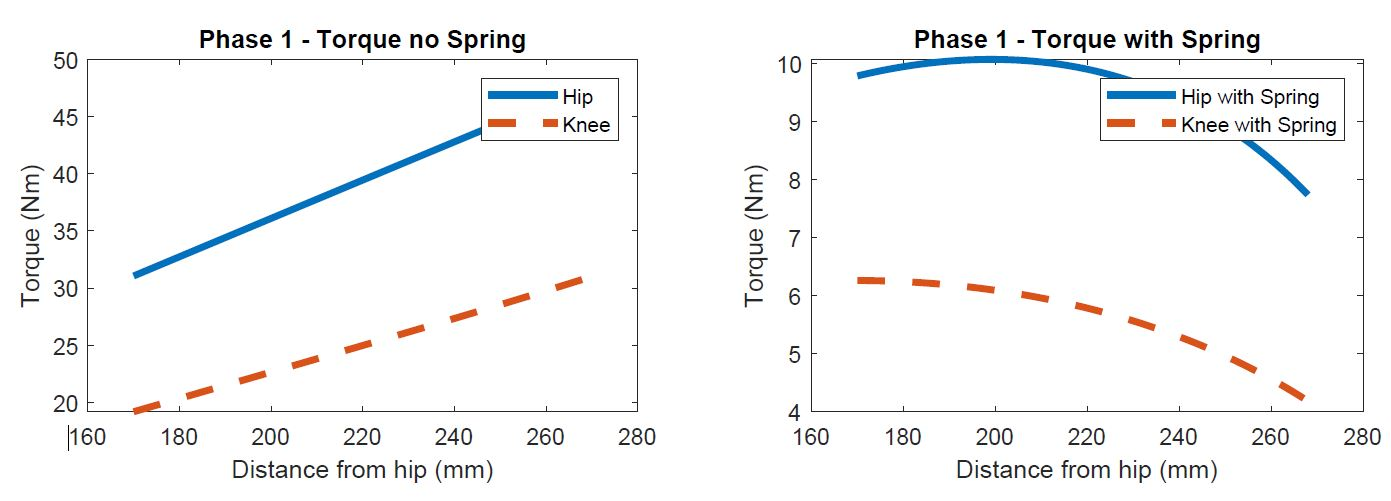
\includegraphics[width=\textwidth]{4_Analysis/img/Spring/SpringVSNoSpring.JPG}
    \caption{Torques before (left) and after (right) the addition of torsion springs on the limbs for the worst phase}
    \label{fig:TorqueB4&after}
\end{figure}

One assumption that deserves to be reviewed is the backdriving torque values for the harmonic drives. In fact, multiple sources state contradicting statements. Therefore, it may be safer to limit the harmonic drives' static torques to values approaching $0 \text{ Nm}$ by setting the spring constant $k$ to obtain approximately the same moment as the maximum static torque.
%------------------------------ Parameterization ------------------------------%
\subsubsection{Parameterization}
One way to parameterize this portion of the analysis could be to input the maximum and minimum torques based on the worst case static analysis along with the spacer diameters and the angular span of both limbs. The backdriving torque of both harmonic drives should be proportionate to the size of the harmonic drive and a safety factor should be set constant. Then, the spring dimensions can be optimized to obtain the smallest springs possible while respecting the spacer diameters, the safety factor, and the required torque.